\subsection{Sequence Diagram}

In the next figures they are illustrated some sequence diagram of the main methods 
\texttt{GET} (figures  \ref{fig:HomePageServlet_doGet}  \ref{fig:BuyProductServlet_doGet}
\ref{fig:InvoiceServlet_doGet} \ref{fig:InvoiceServlet_doGet} \ref{fig:MediaServlet_doGet} \ref{fig:UserServlet_doGet})
and  \texttt{POST}  (figures \ref{fig:LoginServlet_doPost} \ref{fig:MediaServlet_doPost} \ref{fig:UserServlet_doPost}) of the main servlet.

\begin{figure}[H]
    \centering
    \includegraphics[width=\textwidth,height=0.95\textheight,keepaspectratio]{Schemas/HomePageServlet_doGet.svg.pdf}
    \caption{Sequence diagram of \texttt{GET} method of HomePageServlet}
    \label{fig:HomePageServlet_doGet}
\end{figure}

\begin{figure}[H]
    \centering
    \includegraphics[width=\textwidth,height=0.95\textheight,keepaspectratio]{Schemas/BuyProductServlet_doGet.svg.pdf}
    \caption{Sequence diagram of \texttt{GET} method of BuyProductServlet}
    \label{fig:BuyProductServlet_doGet}
\end{figure}

\begin{figure}[H]
    \centering
    \includegraphics[width=\textwidth,height=0.95\textheight,keepaspectratio]{Schemas/InvoiceServlet_doGet.svg.pdf}
    \caption{Sequence diagram of \texttt{GET} method of InvoiceServlet}
    \label{fig:InvoiceServlet_doGet}
\end{figure}
\begin{figure}[H]
    \centering
    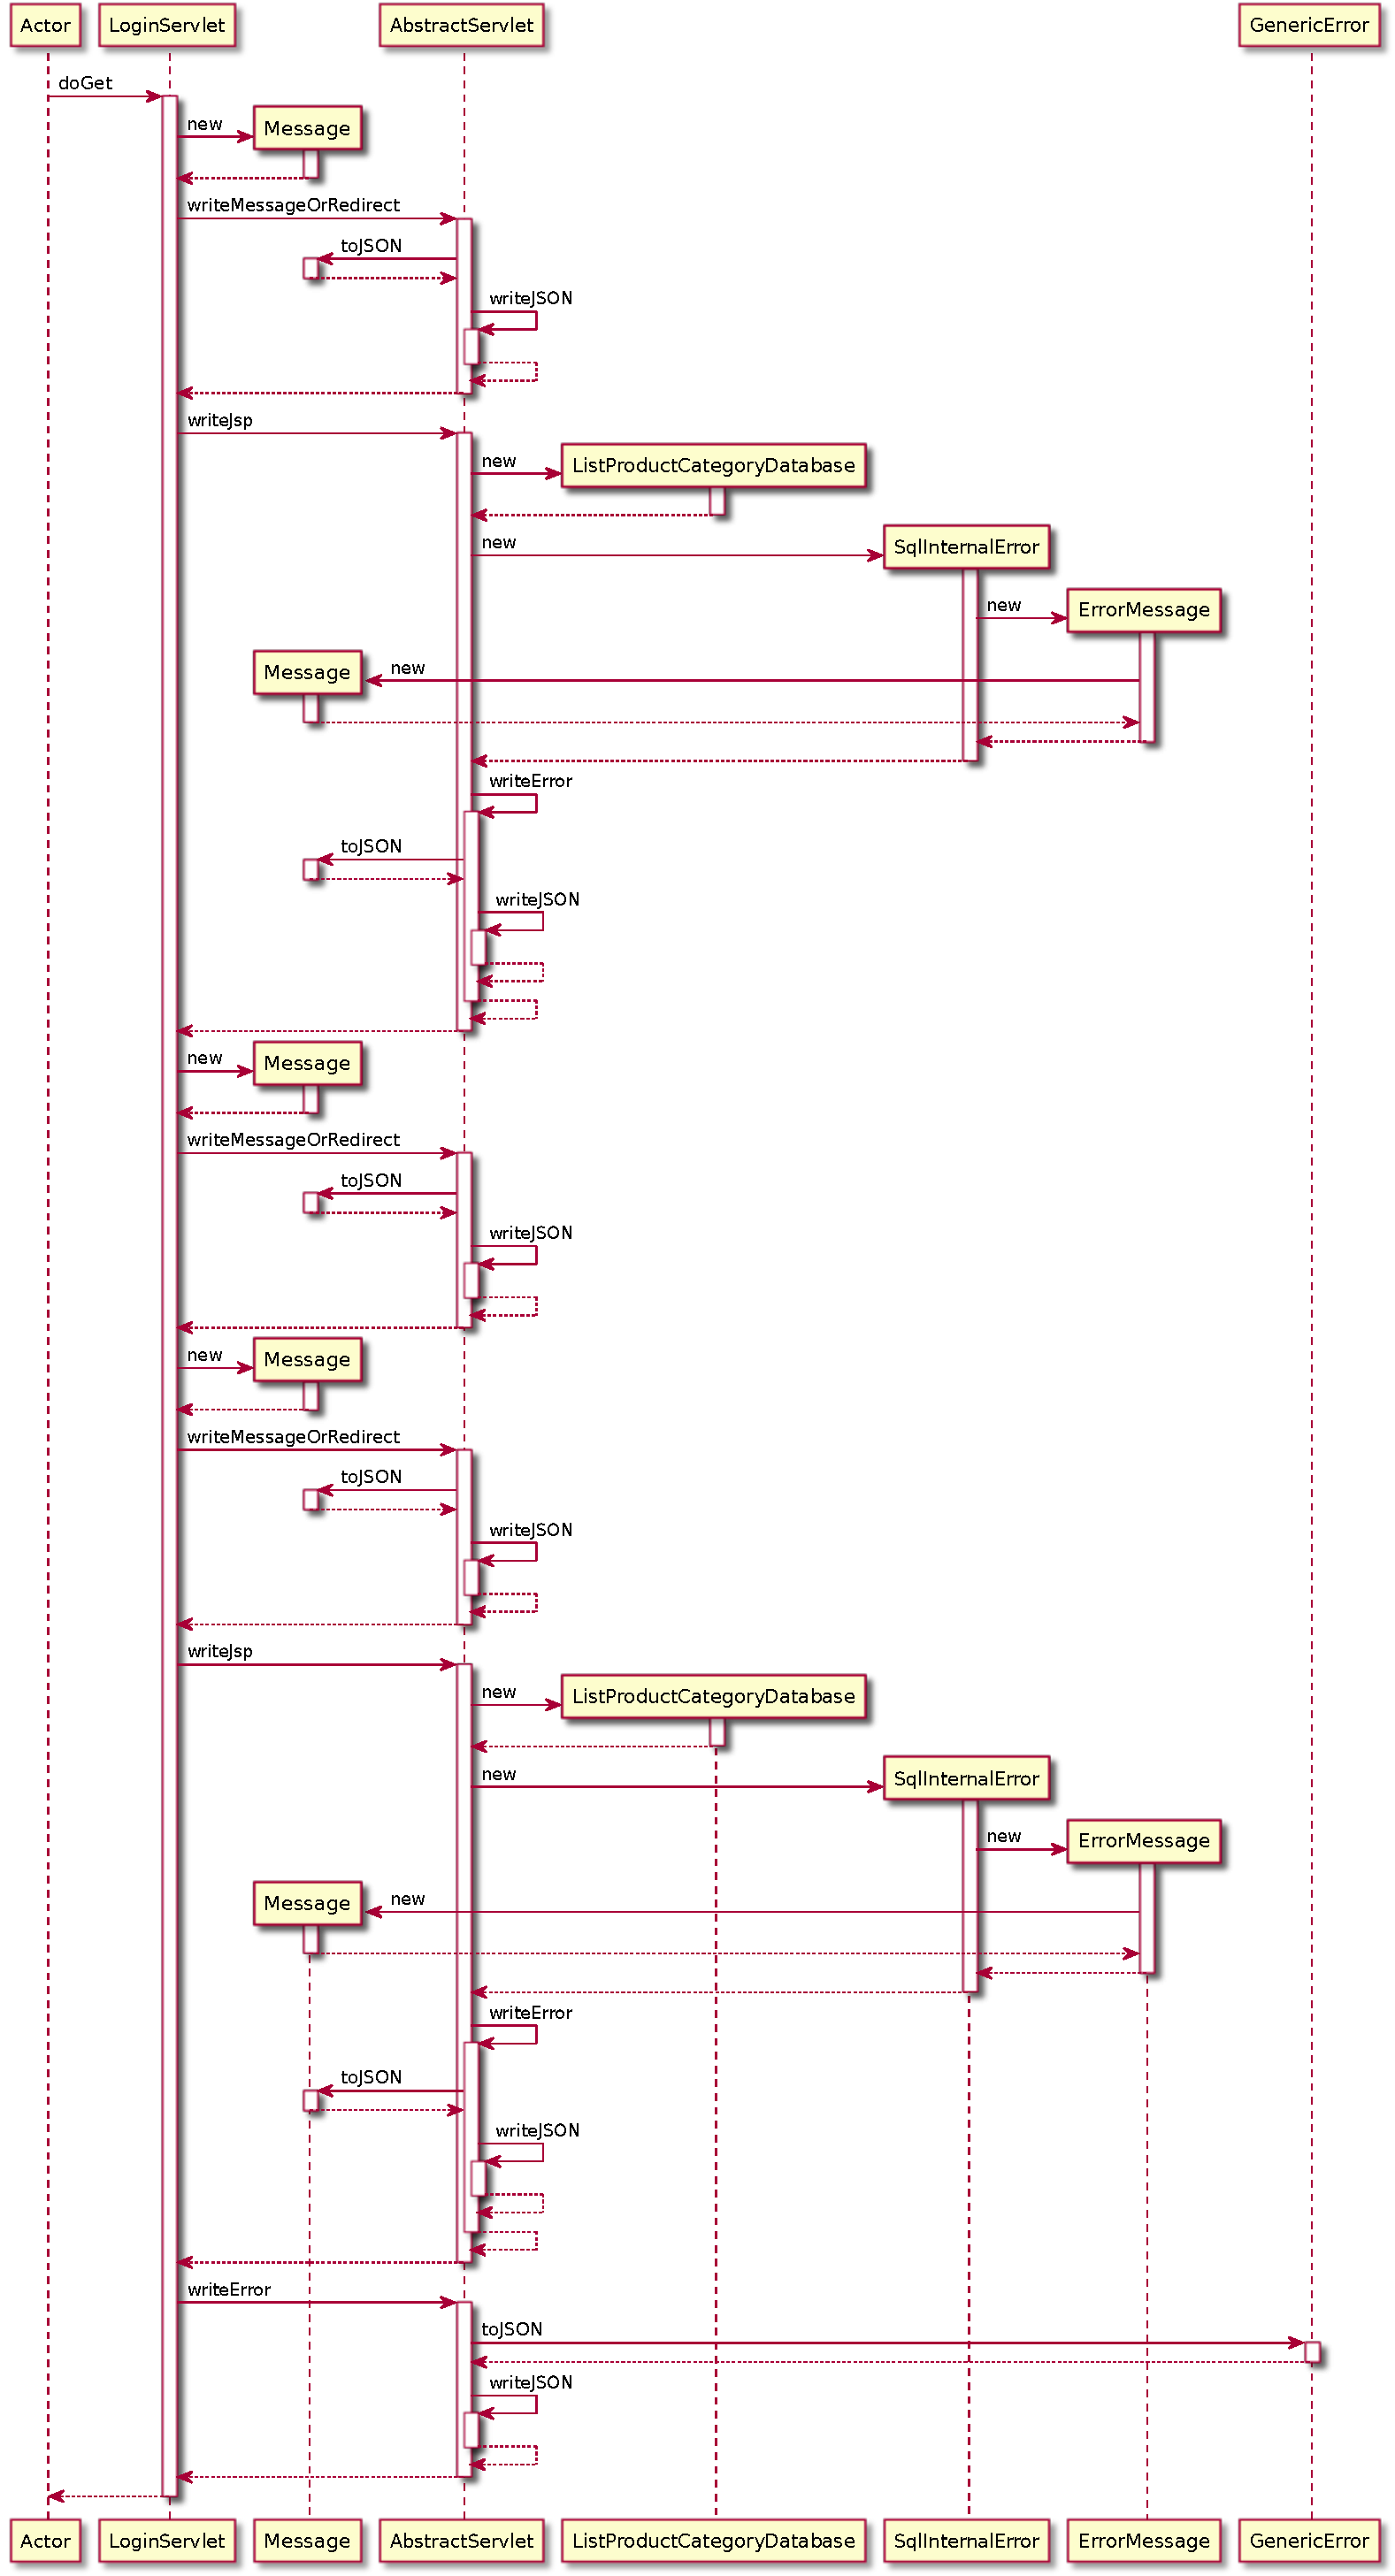
\includegraphics[width=\textwidth,height=0.95\textheight,keepaspectratio]{Schemas/LoginServlet_doGet.svg.pdf}
    \caption{Sequence diagram of \texttt{GET} method of LoginServlet}
    \label{fig:LoginServlet_doGet}
\end{figure}
\begin{figure}[H]
    \centering
    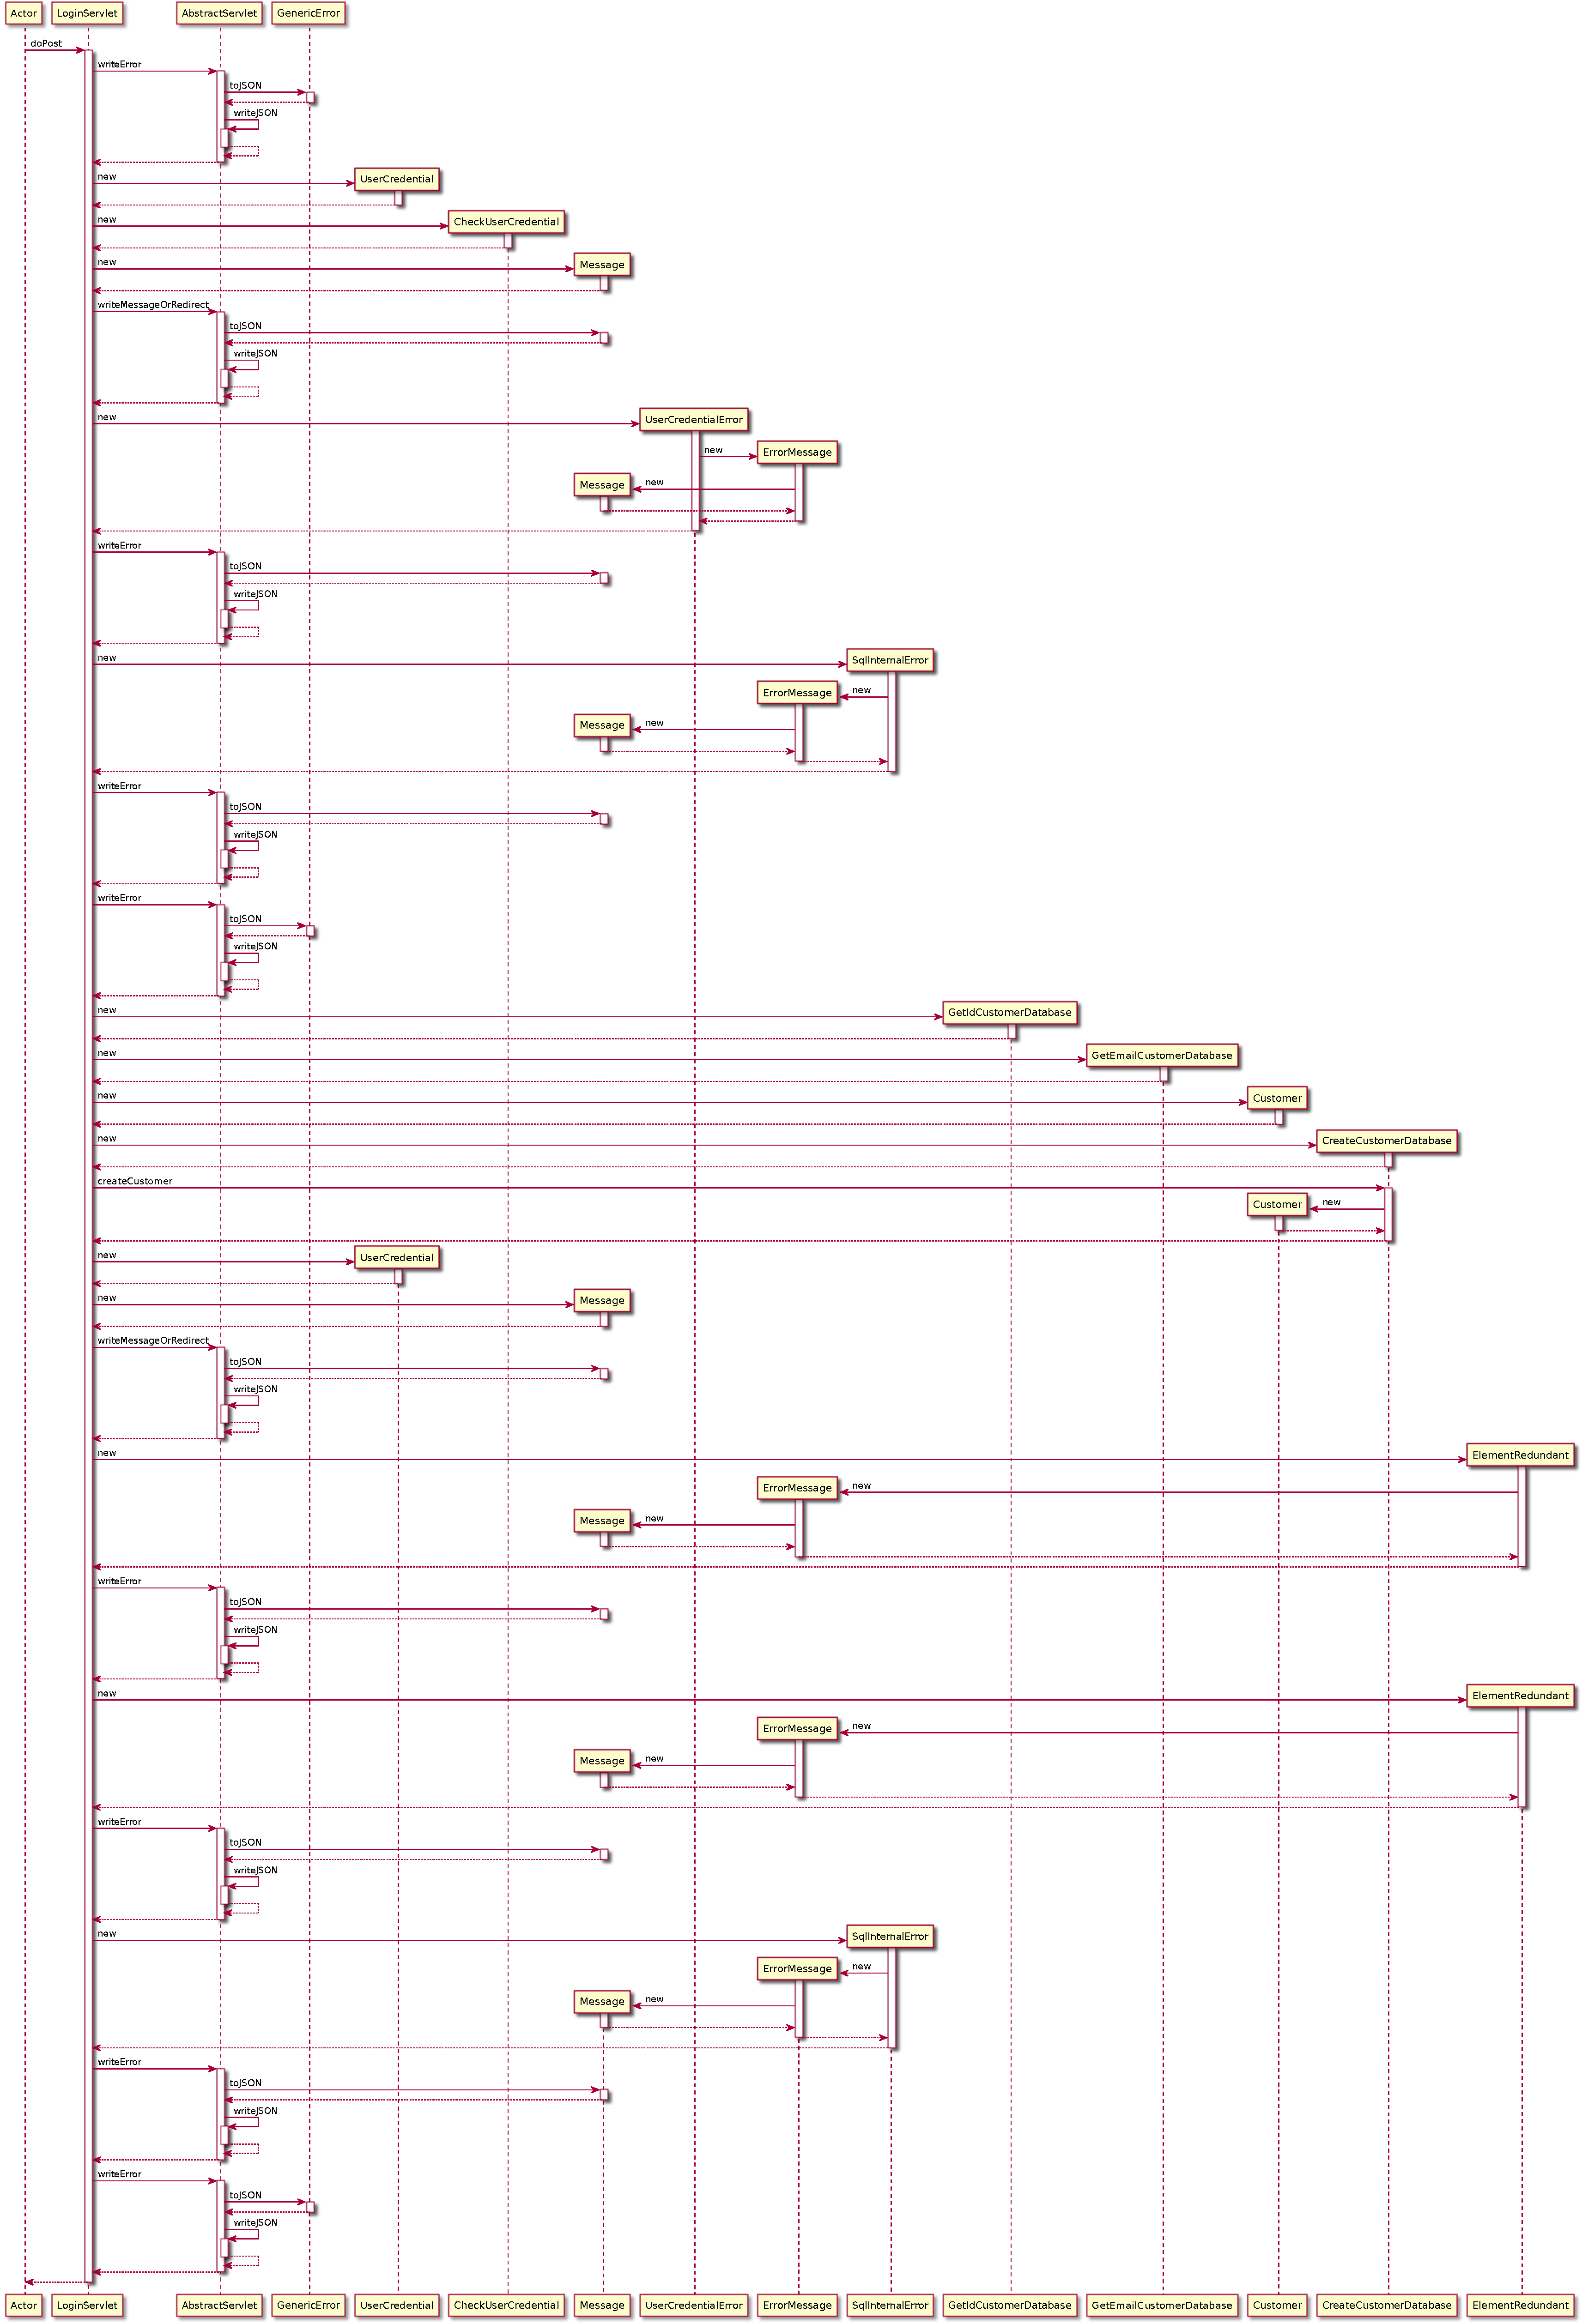
\includegraphics[width=\textwidth,height=0.95\textheight,keepaspectratio]{Schemas/LoginServlet_doPost.svg.pdf}
    \caption{Sequence diagram of \texttt{POST} method of LoginServlet}
    \label{fig:LoginServlet_doPost}
\end{figure}
\begin{figure}[H]
    \centering
    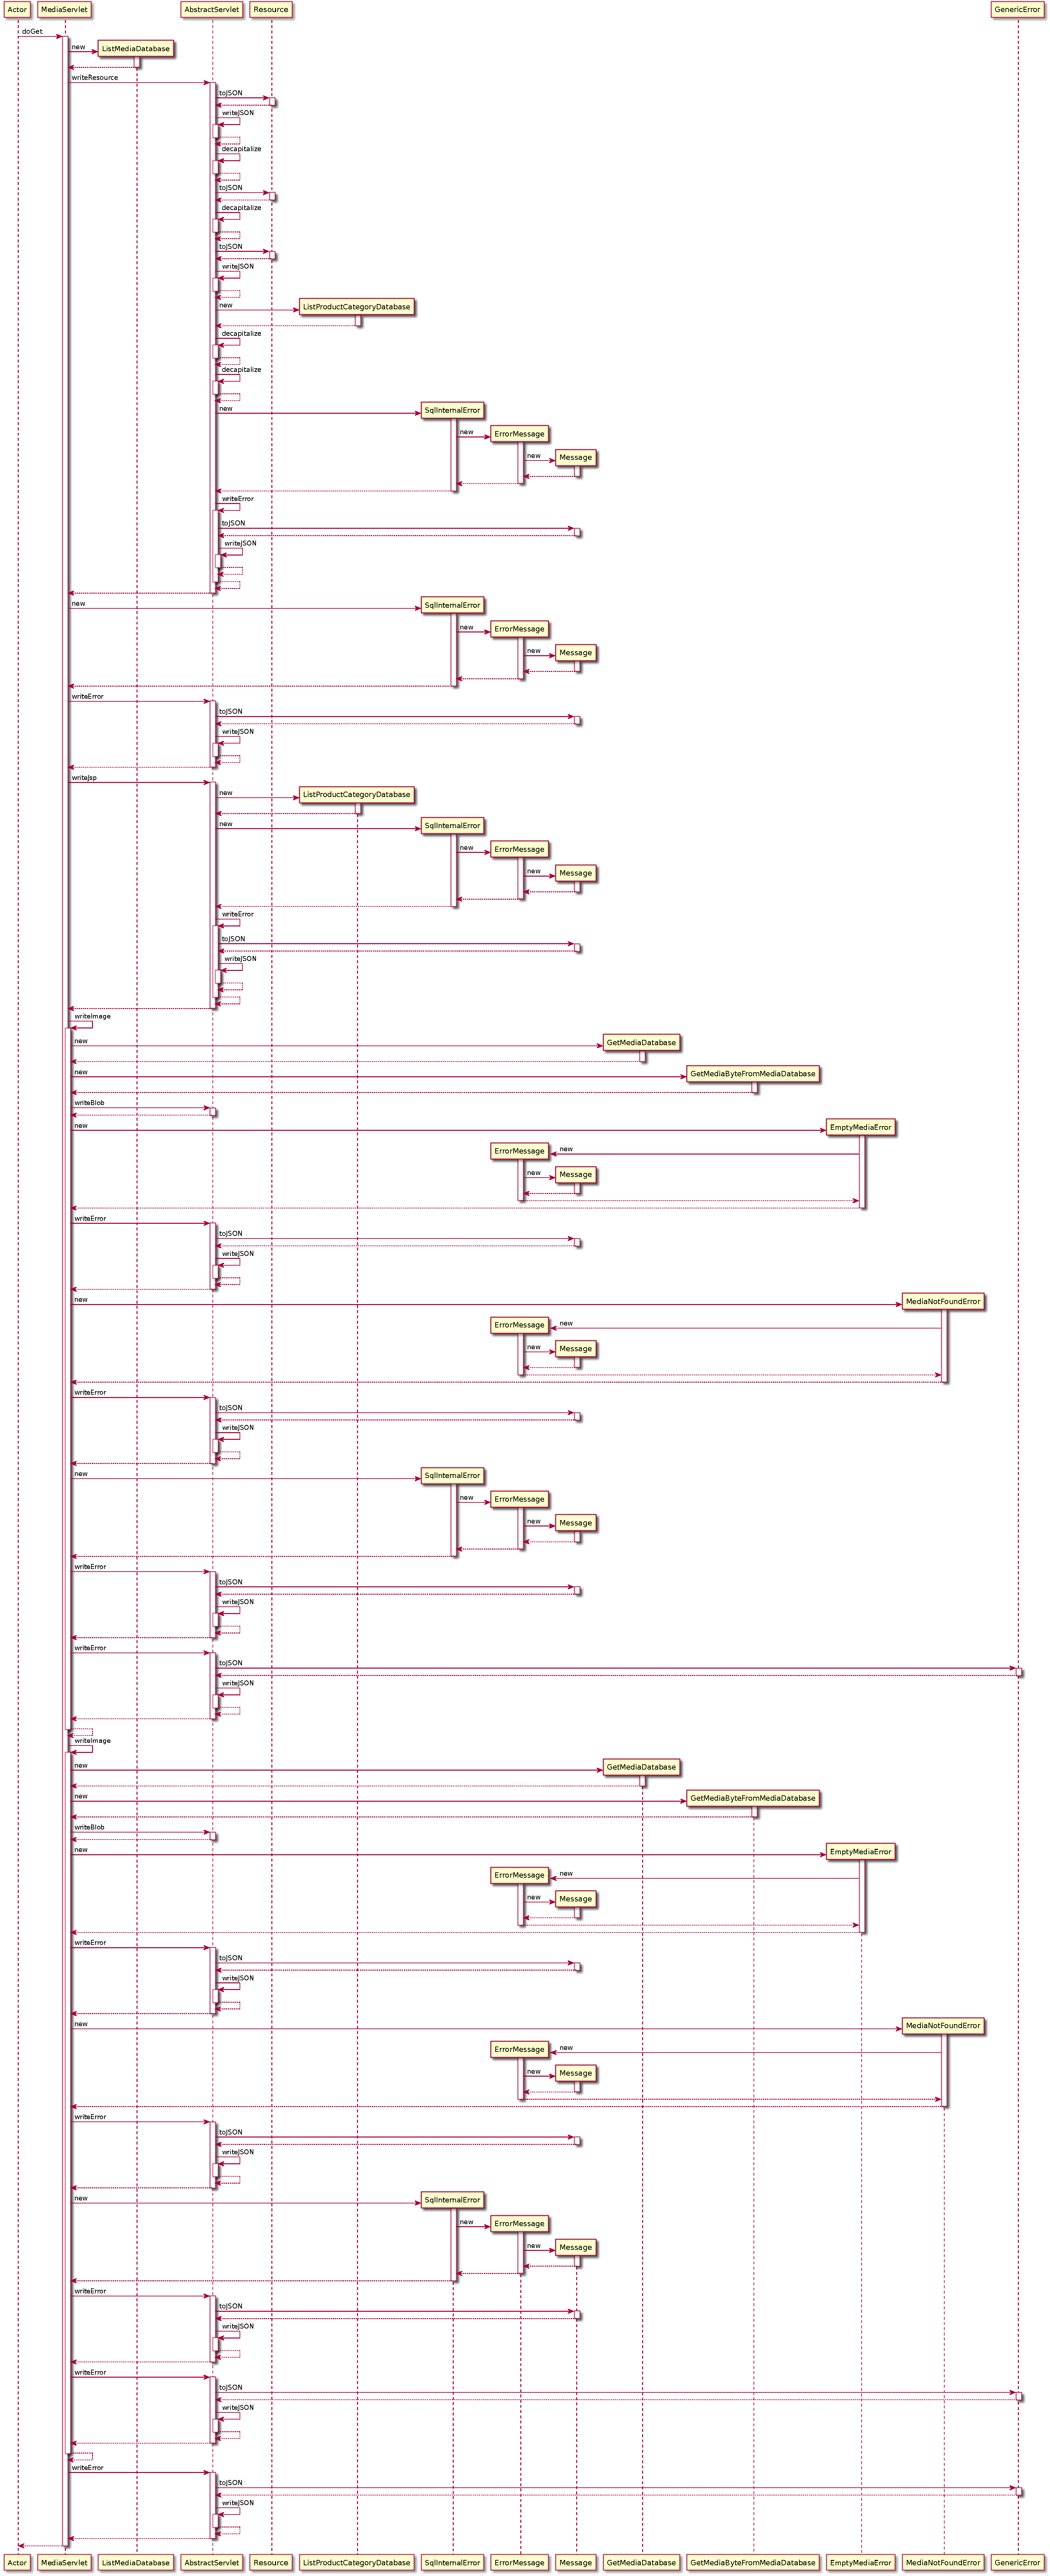
\includegraphics[width=\textwidth,height=0.95\textheight,keepaspectratio]{Schemas/MediaServlet_doGet.svg.pdf}
    \caption{Sequence diagram of \texttt{GET} method of MediaServlet}
    \label{fig:MediaServlet_doGet}
\end{figure}
\begin{figure}[H]
    \centering
    
\includegraphics[width=\textwidth,height=0.95\textheight,keepaspectratio]{Schemas/MediaServlet_doPost.svg.pdf}
    \caption{Sequence diagram of \texttt{POST} method of MediaServlet}
    \label{fig:MediaServlet_doPost}
\end{figure}
\begin{figure}[H]
    \centering
    
\includegraphics[width=\textwidth,height=0.95\textheight,keepaspectratio]{Schemas/UserServlet_doGet.svg.pdf}
    \caption{Sequence diagram of \texttt{GET} method of UserServlet}
    \label{fig:UserServlet_doGet}
\end{figure}
\begin{figure}[H]
    \centering
    \includegraphics[width=\textwidth,height=0.95\textheight,keepaspectratio]{Schemas/UserServlet_doPost.svg.pdf}
    \caption{Sequence diagram of \texttt{POST} method of UserServlet}
    \label{fig:UserServlet_doPost}
\end{figure}

In all the sequence diagrams it is noticed the common characteristic
of the operation of \texttt{writeResource} and \texttt{writeJsp} 
that take care to handle in way uniforms the output.
